\newcommand{\svcourse}{CST Part IA: Introduction to Probability}
\newcommand{\svnumber}{1}
\newcommand{\svvenue}{Churchill, Room TBD}
\newcommand{\svdate}{2022-05-14}
\newcommand{\svtime}{11:00}
\newcommand{\svuploadkey}{PO5ogKIM8KQA22FZS8IAf8gxA8XKi19jxIBVHIfFZ+3GCBXuNUXS9lVN6bNYjxM/}

\newcommand{\svrname}{Mr Matthew Ireland}
\newcommand{\jkfside}{twoside}
\newcommand{\jkfhanded}{right}

\newcommand{\studentname}{Harry Langford}
\newcommand{\studentemail}{hjel2@cam.ac.uk}


\documentclass[10pt,\jkfside,a4paper]{article}

% DO NOT add \usepackage commands here.  Place any custom commands
% into your SV work files.  Anything in the template directory is
% likely to be overwritten!

\usepackage{fancyhdr}

\usepackage{lastpage}       % ``n of m'' page numbering
\usepackage{lscape}         % Makes landscape easier

\usepackage{verbatim}       % Verbatim blocks
\usepackage{epsfig}         % Embed encapsulated postscript
\usepackage{array}          % Array environment
\usepackage[nolinks]{qrcode}         % QR codes
\usepackage{enumitem}       % Required by Tom Johnson's exam question header

\usepackage{hhline}         % Horizontal lines in tables
\usepackage{siunitx}        % Correct spacing of units
\usepackage{amsmath}        % American Mathematical Society
\usepackage{amssymb}        % Maths symbols
\usepackage{amsthm}         % Theorems

\usepackage{ifthen}         % Conditional processing in tex

\usepackage[top=3cm,
            bottom=3cm,
            inner=2cm,
            outer=5cm]{geometry}

% PDF metadata + URL formatting
\usepackage[
            pdfauthor={\studentname},
            pdftitle={\svcourse, SV \svnumber},
            pdfsubject={},
            pdfkeywords={9d2547b00aba40b58fa0378774f72ee6},
            pdfproducer={},
            pdfcreator={},
            hidelinks]{hyperref}

\renewcommand{\headrulewidth}{0.4pt}
\renewcommand{\footrulewidth}{0.4pt}
\fancyheadoffset[LO,LE,RO,RE]{0pt}
\fancyfootoffset[LO,LE,RO,RE]{0pt}
\pagestyle{fancy}
\fancyhead{}
\fancyhead[LO,RE]{{\bfseries \studentname}\\\studentemail}
\fancyhead[RO,LE]{{\bfseries \svcourse, SV~\svnumber}\\\svdate\ \svtime, \svvenue}
\fancyfoot{}
\fancyfoot[LO,RE]{For: \svrname}
\fancyfoot[RO,LE]{\today\hspace{1cm}\thepage\ / \pageref{LastPage}}
\fancyfoot[C]{\qrcode[height=0.8cm]{\svuploadkey}}
\setlength{\headheight}{22.55pt}

\ifthenelse{\equal{\jkfside}{oneside}}{

 \ifthenelse{\equal{\jkfhanded}{left}}{
  % 1. Left-handed marker, one-sided printing or e-marking, use oneside and...
  \evensidemargin=\oddsidemargin
  \oddsidemargin=73pt
  \setlength{\marginparwidth}{111pt}
  \setlength{\marginparsep}{-\marginparsep}
  \addtolength{\marginparsep}{-\textwidth}
  \addtolength{\marginparsep}{-\marginparwidth}
 }{
  % 2. Right-handed marker, one-sided printing or e-marking, use oneside.
  \setlength{\marginparwidth}{111pt}
 }

}{
 % 3. Alternating margins, two-sided printing, use twoside.
}

\setlength{\parindent}{0em}
\addtolength{\parskip}{1ex}

% Exam question headings, labels and sensible layout (courtesy of Tom Johnson)
\setlist{parsep=\parskip, listparindent=\parindent}
\newcommand{\examhead}[3]{\section{#1 Paper #2 Question #3}}
\newenvironment{examquestion}[3]{
    \examhead{#1}{#2}{#3}\setlist[enumerate, 1]{label=(\alph*)}\setlist[enumerate, 2]{label=(\roman*)}
    \marginpar{\qrcode{https://www.cl.cam.ac.uk/teaching/exams/pastpapers/y#1p#2q#3.pdf}}
    \marginpar{\footnotesize \url{https://www.cl.cam.ac.uk/teaching/exams/pastpapers/y#1p#2q#3.pdf}}
}{}



\usepackage{float}
\usepackage{multirow}
\usepackage{multicol}
\usepackage{tikz}
\usepackage{graphicx}

\begin{document}

\section{Lecture 13}

\begin{enumerate}

\item What sort of synchronisation primitives might an atomic fetch-and-add be
useful for?

Logical timestamps.

Whenever a process needs a logical timestamp it can fetch-and-add from a
specified address. The process will then atomically get the current
timestamp and increment the value for the next timestamp.

\item With load linked / store conditional, why does the store alter the
source register containing the value to write?

Store conditional can fail. It fails when the address has been written to
since the load linked. The process needs to know when store conditional has
failed and therefore store conditional needs a return address. One way of
implementing this is to make store-conditional overwrite the value in the
source register with 1 if the store was successful and 0 if it was not. In
RISC-V however, store conditional is explicitly passed a destination register.

\item Assuming a single instruction, \texttt{xchg}, that can do an atomic
exchange of a register and memory location, how would you implement a
na\"{\i}ve spin lock?

\begin{lstlisting}
lock: // spin on the address in x10
	addi t0, x0, 1
	xchg t0, 0(x10)
	beqz t0, lock

unlock: // unlock the address in x10
	addi t0, x0, 0
	xchg t0, 0(x10)
\end{lstlisting}

\item Instead of inefficient spinning on a lock, how might you alter the
lock and unlock code from slide 27 to call routines \texttt{wait\_for\_unlock}
and \texttt{signal\_unlock} to wait when the lock is already taken and
signal other threads once the lock is free?

\begin{lstlisting}
acquire_lock:
	addi t0, x0, 1
	xchg t0, 0(x10)
	bneqz t0, acquired
	addi a0, x0, LOCK // move lock into argument register
	call wait_for_unlock // jal x1, wait_for_unlock
	jmp acquire_lock
acquired:

release_lock:
	addi a0, x0, LOCK // move lock into argument register
	call signal_unlock // jal x1, signal_unlock
\end{lstlisting}

\item What does a memory barrier do?

A memory barrier ensures that all instructions before the memory barrier have
executed and are visible to other cores; and that no instructions after the
memory barrier have been executed.

This is critical for ensuring safety of shared mutable data in processors
with weak consistency.

\item Why do we place a memory barrier after taking a lock and before
releasing the lock, but not the other way round (i.e.\ before taking and
after releasing)?

We place a memory barrier after taking out a lock to prevent the CPU from
executing anything which requires the lock before the lock has been acquired.
If this memory barrier was placed before we took out the lock, then while
spinning the CPU would be able to execute tasks requiring the lock.

Placing a memory barrier before releasing a lock ensures that the lock is
released \textit{after} the thread has finished using it. If it were not
then the thread may release the lock out-of-order and then perform
conflicting operations which required the lock. Placing the memory barrier
after releasing the lock would not prevent this.

\begin{examquestion}{2015}{5}{3}

\begin{enumerate}[label=(\alph*)]

\item

\begin{enumerate}[label=(\roman*)]

\item What are the semantics of load linked and store conditional instructions?

Load linked loads the value of the specified memory.

Store conditional attempts to write a value into the specified memory
address. If the memory address has been written to since the thread loaded
from it using load-linked then the store will fail and will not store and
will only return 0 into the destination register. Otherwise the store will
store and return 1 into the destination register.

\item Describe the synchronisation method that the following code performs
by adding comments to it.

\begin{lstlisting}
	// membar prevents threads syncing out-of-order
	membar
	// load conditional on the lock
label1:
	l1, r2, 0(r1)
	// decrease the count by 1
	sub r2, r2, #1
	// attempt to write back
	sc r2, 0(r1)
	// if the store conditional failed then retry
	beqz r2, label1
	// check how many threads we are waiting on
label2:
	load r2, 0(r1)
	// if this number is nonzero then repeat
	bneq r2, label2
\end{lstlisting}

If the address stored in r1 is initialised to $n$, then the above code will
prevent any thread passing unless exactly $n$ threads are at the same point.
This forces threads to execute in lockstep.

\end{enumerate}

\end{enumerate}

\end{examquestion}

\end{enumerate}

\section{Lecture 14}

\begin{enumerate}

\item Describe SIMT, one way GPUs exploit parallelism. Apart from
performance, what are the other benefits of SIMT execution?

SIMT means single instruction, multiple thread. This is execution of multiple
threads which act on different data and have different state -- but must all
execute the same instruction (or stall waiting for other threads executing
that instruction). This allows for highly parallel execution.

The advantages of SIMT are:

\begin{itemize}

\item Energy efficiency

Since instruction fetch is only performed once per warp and there is minimal
cost associated with deciding which instructions to issue, the amount of
work done per instruction executed is reduced. This increases energy efficiency.

Additionally, GPU cores have less complexity and functionality; making them
more inherently efficient.

\item Uses the data bus less

Since each instruction is only fetched once per warp; the load on the
data bus is reduced. This improves performance on independent processes
which are running on other cores using the same data bus.

\end{itemize}

\item How does the processor pipeline differ from a general-purpose CPU to
allow SIMT execution?

The instruction fetch and instruction decode phases are shared between all
threads in the warp. Therefore each individual core only has the register
fetch, execute, memory access and write-back stages.

\item What are the implications for other parts of the processor for
providing SIMT?

Processors which provide SIMT consume and produce data at a far higher rate.
To support this, DRAM bandwidth must be far higher. Similarly, for SIMT
execution to have any benefit, data must be able to get onto the device.
Loading it in through the CPU and back onto the GPU is not fast enough.
Therefore the GPU must be able to directly access memory -- the CPU must
therefore allow DMA .

SIMT processors typically have very predictable cache access patterns. If
one thread in a warp accesses data then other threads in the warp are likely
to access nearby data. This means that processes which exploit SIMT have
very good spatial locality. The cache should be adapted to take advantage of
this; for example by having significantly larger cachelines. Furthermore, the
cache access patterns will change and so more suitable invalidation
algorithms must be chosen. Since the data we process is far larger, we must
also increase the size of the data cache.

In order to support branching, we need predication -- therefore every
core must have a predicate register and the ability to invalidate instructions.

The processor needs more ALUs and registers on which to execute all the
threads in parallel.

SIMT execution will use energy and create heat. This means there is less
energy and heat dissipation available for the rest of the processor.
Therefore the rest of the processor must operate at a lower clock rate or
otherwise use less energy to function properly and avoid overheating.

\item What is the basic way GPUs allow branching within the different threads?

My interpretation of ``the basic way'' does not any optimisations (ie
skipping conditional statements if no threads in a warp execute them) or
involve nested branches (for which we would need a stack of predicates).

GPUs emulate branching by predication. In predication, the value of a
predicate is evaluated at the start conditional code. This is written into a
``predicate register''. Instructions then check the predicate register
before committing -- if the instruction is not meant to be executed then it
should not commit. At the end of the if statement, the predicates are
inverted for the else statement. At the end of the else statement the
predicate register is reset to allow all threads to execute.

All threads in a warp execute in lockstep -- they execute the same
instruction at once. This means threads cannot simply ``skip'' a branch and
leads to inefficient solutions such as predication; where every thread
which does not take a branch will stall until the end of a branch.

\begin{enumerate}[label=(\alph*)]

\item What does this imply about the way you should write code for GPUs?

Code written for GPUs should have as little conditional execution as
possible. Any conditional code we do write should be as short as possible.

\item Why does it make sense to do as little work as possible within the
target of an infrequently-taken branch?

If no thread in a warp executes a branch then all threads in that warp will
stall for the number of cycles required to execute that conditional
statement (excluding time for ie memory accesses). If there is a long
infrequently-taken branch then the GPU will stall for significant amounts of
time. Consider a executing 1000 instructions on a GPU which contains 500
instructions which only 1\% of threads will execute. This one branch has
reduced efficiency down to 50.5\%.

\end{enumerate}

\item Assuming each line below is a single instruction, what is the
efficiency of the code?

\begin{lstlisting}[numbers=left]
ld X[i:i+3]
if (i % 2 == 0)
	mul a, X[i:i+3]
else
	mul b, X[i:i+3]
	if (i % 4 == 1)
		add c, X[i:i+3]
		mul 2, x{i:i+3]
	endif
endif
\end{lstlisting}

The efficiency of the code is the average proportion of threads which
execute each instruction which is fetched.

I define efficiency as the number of useful instructions executed divided by
the total number of cycles across all cores. This considers control
instructions ie endif, else as inefficient (rewarding control instructions
is not reasonable). We can approximate this by using the probability of an
instruction being executed divided by the number of cycles.

\[
e = \frac{\sum^{n}_{i=1} p_i}{n}
\]

Lines 1 and 2 will be executed by all threads. line 3 will be executed by
half of threads, lines 5 and 6 will be executed by half of threads and lines
7 and 8 will be executed by a quarter of threads. All other lines are
control structures dependent on our specific implementation and do not do
``useful'' work.

Therefore the efficiency is given by:
\[
\begin{split}
e
&= \frac{1 + 1 + \frac{1}{2} + \frac{1}{2} + \frac{1}{2} + \frac{1}{4} +
\frac{1}{4}}{10} \\
&= \frac{3}{10} \\
\end{split}
\]

\item Why do GPUs rely on parallelism between warps as well as SIMT? What
bottleneck does this target?

GPUs process large amounts of data. Since threads execute in lockstep, if any
thread in the warp has a cache miss, all threads in the warp are forced
to stall. GPUs have intentionally small caches and therefore cache misses are
comparatively frequent. Furthermore, GPUs are physically far away from DRAM
or main memory and therefore data fetches take a long time. To mitigate this
the GPU relies on parallelism between warps and will start executing
another warp while the memory access takes place.

This targets the von neumann bottleneck.

\item How can a SIMT processor pipeline be modified the extract parallelism
between warps?

In order to support parallelism between warps, the SIMT processor must
support multithreading. This requires a scheduler (known as the warp
scheduler) which will issue instructions where all the operands are
available and hence can execute. The cores themselves must also support
multithreading -- therefore they will need duplicate registers to hold the
register values for each warp which is being multithreaded. Furthermore, we
will need to adapt the processor such that it does not stall unnecessarily
 -- the scheduler will only issue instructions where the operands are ready
and therefore the core does not need to stall elsewhere.

\item The warp scheduler chooses instructions to execute. What are its
criteria for choosing and what other schemes could be implemented?

The warp scheduler considers the availability of the operands for each
instruction. If the operands for an instruction are not ready, then the
instruction will not be issued.

However, the warp scheduler could be extended to take account of priority:
for example we could set the priority to be the importance of warps or
the number of instructions remaining (to ensure warps are executed as
quickly as possible) -- or the number of blocking reads the warp has left.

\end{enumerate}

\begin{examquestion}{2016}{5}{3}

\begin{enumerate}[label=(\alph*)]

\setcounter{enumi}{1}

\item Consider the following pseudocode that is run on a SIMD processor with
8 lanes where \texttt{i} gives the lane number.

\begin{lstlisting}[numbers=left]
r1 = load X[i]
r2 = load Y[i]
if (i % 2 == 0)
	if (i % 8 == 0)
		r1 = r1 * 2
		r1 = r1 + r2
	endif
else
	r1 = r1 - r2
endif
store r1, X[i]
\end{lstlisting}

\begin{enumerate}[label=(\roman*)]

\item Describe how the processor can support branch divergence between the
different lanes.

Each lane has a predicate register. This register holds 1 if the current
instruction should be executed and 0 if it should not. On branching, lanes
evaluate predicates and if the predicate is false, set their predicate
register to 1. In the write-back and memory access stage, the thread will
check whether the predicate register is set. If it is, then the instruction
will commit. Otherwise it will not commit. This ensures that instructions
commit if and only if they are meant to and enables branch divergence.

\item With the aid of a diagram, show the utilisation of the SIMD lanes for
each pseudocode operation, hence calculate the code's efficiency.

\begin{table}[H]
\centering
\begin{tabular}{l l|l l l l l l l l}
& & \multicolumn{7}{c}{instruction} \\
& & 1 & 2 & 3 & 4 & 5 & 6 & 8 & 11\\
\hline
\multirow{8}{*}{Lane}
& 0 & \checkmark & \checkmark & \checkmark & \checkmark & \checkmark &
\checkmark & \checkmark \\
& 1 & \checkmark & \checkmark & \checkmark & & & & \checkmark & \checkmark \\
& 2 & \checkmark & \checkmark & \checkmark & \checkmark & & & & \checkmark \\
& 3 & \checkmark & \checkmark & \checkmark & & & & \checkmark & \checkmark \\
& 4 & \checkmark & \checkmark & \checkmark & \checkmark & & & & \checkmark \\
& 5 & \checkmark & \checkmark & \checkmark & & & & \checkmark & \checkmark \\
& 6 & \checkmark & \checkmark & \checkmark & \checkmark & & & & \checkmark \\
& 7 & \checkmark & \checkmark & \checkmark & & & & \checkmark & \checkmark \\
\end{tabular}
\end{table}

Once again, I use the ``moral'' definition of efficiency; which considers
control instructions as inefficient.

Out of $11 \cdot 8 = 88$ cycles taken, only 42 are used. Therefore the
efficiency of the code is $\frac{42}{88} = \frac{17}{28} \approx 0.477$.

\item What architectural technique to GPUs employ to allow them to perform
useful work even though the loads from \texttt{X} and \texttt{Y} often cause
stalls?

GPUs exploit multithreading to mitigate the effect of stalls. The warp
scheduler holds information about when the operands for each instruction in
each warp are ready. If there is an instruction which could be executed, the
warp scheduler will issue this instruction. This ensures that the GPU never
stalls when there is work that could be done and increases overall utilisation.

\end{enumerate}

\end{enumerate}

\end{examquestion}

\begin{examquestion}{2019}{5}{3}

\begin{enumerate}[label=(\alph*)]

\setcounter{enumi}{3}

\item Describe, with the aid of a diagram how a GPU executes data-parallel
kernels efficiently, including the two main pieces of hardware support.

GPUs consist of a large array of cores which all operate on different
threads from the same program. Each of these cores are relatively weak, but
GPUs focus on throughput via parallelisation and therefore the power of each
individual core is not significant. The diagram below demonstrates how much
of the core is processed in parallel: the dark green is compute while light
green, blue and orange signify data. Compared to a CPU this demonstrates a
very high proportion of the chip dedicated to computation.

\begin{figure}[H]
\centering
\includegraphics[width=0.5\textwidth]{./fermi_gpu}
\end{figure}

Furthermore, notice the DRAM sockets. Since GPUs are so fast, they process a
large amount of data and therefore to enable a GPU to process data rapidly,
the data must be provided. This is usually done by increasing the number of
DRAM ports and width of the data bus such that enough data can be sent to
the GPU .

\iffalse

\begin{center}

\begin{tikzpicture}

\draw[-stealth, thick] (-0.5, 0) -- (-0.5, -6.5);
\node[anchor=east] at (-0.75, -3.25) {Time};
\draw[-stealth] (1.75, -0.5) -- (1.75, -1);
\draw[-stealth] (1.75, -1.5) -- (1.75, -2);
\draw[-stealth] (1.75, -2.5) -- (1.75, -3);
\draw[-stealth] (1.75, -3.5) -- (1.75, -4);
\draw[-stealth] (1.75, -4.5) -- (1.75, -5);
\draw[-stealth] (1.75, -5.5) -- (1.75, -6);

\draw[rounded corners=1mm] (0, 0) rectangle (3.5, -0.5);
\node[anchor=center] at (1.75, -0.25) {Warp 1 Instruction 1};
\draw[rounded corners=1mm] (0, -1) rectangle (3.5, -1.5);
\node[anchor=center] at (1.75, -1.25) {Warp 1 Instruction 2};
\node[anchor=west] at (4, -1.25) {Stall};
\draw[-stealth] (4, -1.25) -- (3.55, -1.25);
\draw[rounded corners=1mm] (0, -2) rectangle (3.5, -2.5);
\node[anchor=center] at (1.75, -2.25) {Warp 2 Instruction 1};
\node[anchor=west] at (4, -2.25) {Stall};
\draw[-stealth] (4, -2.25) -- (3.55, -2.25);
\draw[rounded corners=1mm] (0, -3) rectangle (3.5, -3.5);
\node[anchor=center] at (1.75, -3.25) {Warp 3 Instruction 1};
\draw[rounded corners=1mm] (0, -4) rectangle (3.5, -4.5);
\node[anchor=center] at (1.75, -4.25) {Warp 3 Instruction 2};
\node[anchor=west] at (4, -4.25) {Stall};
\draw[-stealth] (4, -4.25) -- (3.55, -4.25);
\draw[rounded corners=1mm] (0, -5) rectangle (3.5, -5.5);
\node[anchor=center] at (1.75, -5.25) {Warp 1 Instruction 3};
\draw[rounded corners=1mm] (0, -6) rectangle (3.5, -6.5);
\node[anchor=center] at (1.75, -6.25) {Warp 1 Instruction 4};

\end{tikzpicture}

\begin{tikzpicture}
\draw[rounded corners=1mm] (0, 0) rectangle (6, 3.8);
\node[anchor=center] at (3, 3.4) {Core 2};
\draw[rounded corners=1mm] (0.2, 0.2) rectangle (5.8, 0.9);
\node[anchor=center] at (3, 0.55) {ALU};
\draw[rounded corners=1mm] (0.2, 1.1) rectangle (2.9, 1.9);
\node[anchor=center] at (1.55, 1.5) {Register file 3};
\draw[rounded corners=1mm] (0.2, 2.1) rectangle (2.9, 2.9);
\node[anchor=center] at (1.55, 2.5) {Register file 1};
\draw[rounded corners=1mm] (3.1, 1.1) rectangle (5.8, 1.9);
\node[anchor=center] at (4.45, 2.5) {Register file 2};
\draw[rounded corners=1mm] (3.1, 2.1) rectangle (5.8, 2.9);
\node[anchor=center] at (4.45, 1.5) {Register file 4};

\draw[rounded corners=1mm] (7, 0) rectangle (13, 3.8);
\node[anchor=center] at (10, 3.4) {Core 2};
\draw[rounded corners=1mm] (7.2, 0.2) rectangle (12.8, 0.9);
\node[anchor=center] at (10, 0.55) {ALU};
\draw[rounded corners=1mm] (7.2, 1.1) rectangle (9.9, 1.9);
\node[anchor=center] at (8.55, 1.5) {Register file 3};
\draw[rounded corners=1mm] (7.2, 2.1) rectangle (9.9, 2.9);
\node[anchor=center] at (8.55, 2.5) {Register file 1};
\draw[rounded corners=1mm] (10.1, 1.1) rectangle (12.8, 1.9);
\node[anchor=center] at (11.45, 2.5) {Register file 2};
\draw[rounded corners=1mm] (10.1, 2.1) rectangle (12.8, 2.9);
\node[anchor=center] at (11.45, 1.5) {Register file 4};
\end{tikzpicture}

\end{center}

The two main pieces of hardware support for data-parallel execution are the
warp scheduler and the multiple sets of registers. The warp scheduler
chooses which warp the execute based on the set of warps which are ready.
This scheduling algorithm chosen can be arbitrarily complicated. This
ensures high utilisation. Each core also needs multiple sets of registers to
allow it to store the state for the thread that executed on that core in each
warp which could be stalled.

\fi

\item Describe the trade-offs between using a GPU or a specialised
accelerator for tasks containing data-level parallelism.

Using a GPU or specialised hardware accelerator means execution time can be
dramatically reduced. Since these devices are designed specifically for the
task, they will implement minimal additional functionality and may be able
to exploit massive parallelism which cannot be obtained on a normal CPU .
Furthermore, since the accelerators are designed for one task in mind they can
be significantly more energy efficient. Accelerators which exploit large
parallelism may additionally have simpler cores which further increase
energy efficiency.

However, accelerators are physically large and distant from the main CPU .
This means that moving data onto an accelerator can add significant overhead;
therefore making them unsuitable for small jobs.

Furthermore, most accelerators rely on data independent threads to take
advantage of parallelism. Therefore if the threads are not data-independent
we cannot use an accelerator efficiently.

Additionally, GPUs and other accelerators execute instructions in lockstep --
so if one instruction gets blocked then all instructions in the warp will
also be blocked. Threads in the same warp must also wait for all threads in
the same warp which take conditional branches.

\end{enumerate}

\end{examquestion}

\end{document}
